% This file was created by matlab2tikz.
%
%The latest updates can be retrieved from
%  http://www.mathworks.com/matlabcentral/fileexchange/22022-matlab2tikz-matlab2tikz
%where you can also make suggestions and rate matlab2tikz.
%
\definecolor{mycolor1}{rgb}{0.00000,0.44700,0.74100}%
%
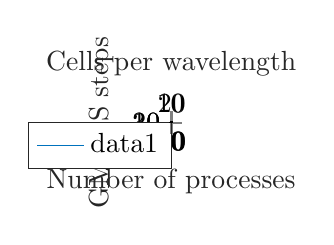
\begin{tikzpicture}

\begin{axis}[%
width=0.951\fwidth,
height=0.33\fwidth,
at={(0\fwidth,0\fwidth)},
scale only axis,
xmin=7,
xmax=81,
xlabel style={font=\color{white!15!black}},
xlabel={Number of processes},
ymin=5,
ymax=35,
ylabel style={font=\color{white!15!black}},
ylabel={GMRES steps},
axis background/.style={fill=white},
axis x line*=bottom,
axis y line*=left,
legend style={legend cell align=left, align=left, draw=white!15!black}
]
\addplot [color=mycolor1]
  table[row sep=crcr]{%
8	20\\
12	16\\
16	32\\
20	22\\
24	10\\
28	8\\
32	7\\
36	7\\
40	9\\
56	10\\
80	24\\
};
\addlegendentry{data1}

\end{axis}

\begin{axis}[%
width=0.951\fwidth,
height=0.33\fwidth,
at={(0\fwidth,0\fwidth)},
scale only axis,
xmin=3,
xmax=26,
xlabel style={font=\color{white!15!black}},
xlabel={Cells per wavelength},
ymin=1,
ymax=10,
ytick={\empty},
axis x line*=top,
axis y line*=left,
legend style={legend cell align=left, align=left, draw=white!15!black, fill=white!94!black}
]
\end{axis}
\end{tikzpicture}%